\documentclass{article}
\usepackage{fullpage}
\usepackage{amsmath}
\usepackage{amsfonts}
\usepackage{authblk}
\usepackage{titling}
\usepackage{tikz}

\title{\huge{Classical Mechanics 1, Autumn 2021 CMI \\ Problem set 1\\\hspace{7cm}- Govind S. Krishnaswami}
}
\author{Soham Chatterjee\\Roll: BMC202175}
\date{}


\renewcommand\maketitlehooka{\null\mbox{}\vfill}
\renewcommand\maketitlehookd{\vfill\null}

\setlength{\parindent}{1cm}
\begin{document}
	\maketitle
	\pagebreak
	\begin{enumerate}
		\item \textbf{\underline{Geometric Interpretation of Non-collinear  Vector Subtraction}:-}
		
		\hspace{1cm}Let $\vec{A}$ and $\vec{B}$ are two non-collinear vectors emanating from origin in $2d$ plane which makes an angle $\theta$ with each other.
		
		\begin{center}
			\begin{tikzpicture}
			\draw[->] (0,0) node[xshift=0.7cm,yshift=1.5cm] {$\vec{A}$} -- (2,3);
			\draw[->] (0,0) node[xshift=2cm,yshift=-0.3cm] {$\vec{B}$} -- (4,0);
			\draw (1,0) arc [start angle=0, end angle=55, radius=1cm] node[xshift=0.5cm,yshift=-0.3cm] {$\theta$};
			\end{tikzpicture}
		\end{center}
		\hspace{1cm}Now for $\vec{A}-\vec{B}$ we can write this as $\vec{A}+(-\vec{B})$ where $-\vec{B}$ represents the vector which has same magnitude as $\vec{B}$ but the direction is oppesite. Hence this $-\vec{B}$ vector makes an agle $180^{\circ}-\theta$ with $\vec{A}$
		
		\begin{center}
			\begin{tikzpicture}
				\draw[->] (0,0) node[xshift=0.7cm,yshift=1.5cm] {$\vec{A}$} -- (2,3);
				\draw[->] (0,0) node[xshift=2cm,yshift=-0.3cm] {$\vec{B}$} -- (4,0);
				\draw (1,0) arc [start angle=0, end angle=55, radius=1cm] node[xshift=0.5cm,yshift=-0.3cm] {$\theta$};
				\draw[->] (0,0) node[xshift=-2cm,yshift=-0.3cm] {$-\vec{B}$} -- (-4,0);
				\draw (-1,0) arc [start angle=180, end angle=65, radius=1.2cm] node[xshift=-2.3cm,yshift=-0.3cm] {$180^{\circ}-\theta$};
			\end{tikzpicture}
		\end{center}
		Now addition of this two vectors will be the diagonal of the parallelogram whose two adjacent sides are $\vec{A}$ and $-\vec{B}$.
		
		\begin{center}
			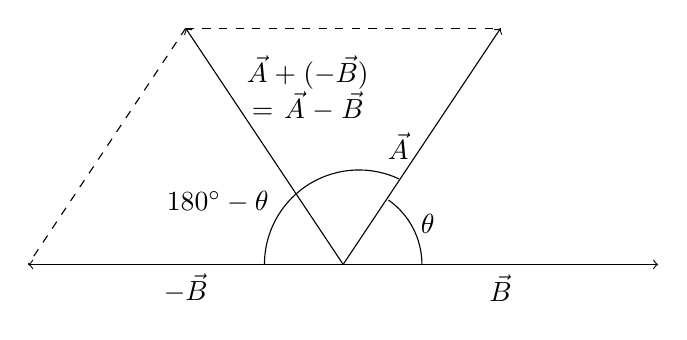
\begin{tikzpicture}
				\draw[->] (0,0) node[xshift=0.7cm,yshift=1.5cm] {$\vec{A}$} -- (2,3);
				\draw[->] (0,0) node[xshift=2cm,yshift=-0.3cm] {$\vec{B}$} -- (4,0);
				\draw (1,0) arc [start angle=0, end angle=55, radius=1cm] node[xshift=0.5cm,yshift=-0.3cm] {$\theta$};
				\draw[->] (0,0) node[xshift=-2cm,yshift=-0.3cm] {$-\vec{B}$} -- (-4,0);
				\draw (-1,0) arc [start angle=180, end angle=65, radius=1.2cm] node[xshift=-2.3cm,yshift=-0.3cm] {$180^{\circ}-\theta$};
				\draw[dashed] (-2,3) -- (2,3);
				\draw[dashed] (-2,3) -- (-4,0);
				\draw[->] (0,0) node[xshift=-0.45cm,yshift=1.7cm,above,text width=2cm,align=center] {$\vec{A}+(-\vec{B})$
					 $=\vec{A}-\vec{B}$} -- (-2,3);
			\end{tikzpicture}
		\end{center}
		Hence we can say geometrically that $\vec{A}-\vec{B}$ is the third side of the triangle made by $\vec{A}$ and $-\vec{B}$.
		
		\begin{center}
			\begin{tikzpicture}
				\draw[->] (-4,0) node[xshift=0.7cm,yshift=1.5cm] {$\vec{A}$} -- (-2,3);
				\draw[->] (0,0) node[xshift=-2cm,yshift=-0.3cm] {$-\vec{B}$} -- (-4,0);
				\draw[dashed] (-2,3) -- (-4,0);
				\draw[->] (0,0) node[xshift=-0.45cm,yshift=1.7cm,above,text width=2cm,align=center] {$\vec{A}-\vec{B}$} -- (-2,3);
			\end{tikzpicture}
		\end{center}
		\item  Let $\textbf{a}$ and $\textbf{b}$ are two  vectors in $\mathbb{R}^3$ which makes an angle $\theta$ with each other.
		\begin{center}
			\begin{tikzpicture}
				\draw[->] (0,0) node[xshift=0.7cm,yshift=1.5cm] {$\textbf{a}$} -- (2,3);
				\draw[->] (0,0) node[xshift=2cm,yshift=-0.3cm] {$\textbf{b}$} -- (4,0);
				\draw (1,0) arc [start angle=0, end angle=56, radius=1cm] node[xshift=0.5cm,yshift=-0.3cm] {$\theta$};
			\end{tikzpicture}
		\end{center}
		Hence the the vector $\textbf{c}=\textbf{a}+\textbf{b}$ is the resultant vector 
		
		\begin{center}
			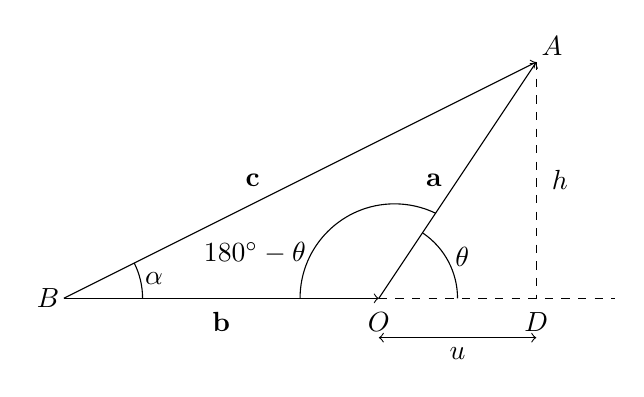
\begin{tikzpicture}
				\draw[->] (4,0) node[xshift=0.7cm,yshift=1.5cm] {$\textbf{a}$} -- (6,3);
				\draw[->] (0,0) node[xshift=2cm,yshift=-0.3cm] {$\textbf{b}$} -- (4,0);
				\draw[dashed] (4,0) -- (7,0);
				\draw (5,0) arc [start angle=0, end angle=56, radius=1cm] node[xshift=0.5cm,yshift=-0.3cm] {$\theta$};
				\draw[->] (0,0) node[xshift=2.4cm,yshift=1.5cm] {$\textbf{c}$} -- (6,3);
				\draw[dashed] (6,3) node[xshift=0.3cm,yshift=-1.5cm] {$h$} -- (6,0);
				\draw (3,0) arc [start angle=180, end angle=64, radius=1.2cm] node[xshift=-2.3cm,yshift=-0.5cm] {$180^{\circ}-\theta$};
				\draw (0,0) node[xshift=-0.2cm] {$B$};
				\draw (6,3) node[xshift=0.2cm,yshift=0.2cm] {$A$};
				\draw (4,0) node[yshift=-0.3cm] {$O$};
				\draw (6,0) node[yshift=-0.3cm] {$D$};
				\draw[<->] (4,-0.5) node[xshift=1cm,yshift=-0.2cm] {$u$} -- (6,-0.5);
				\draw (1,0) arc [start angle=0, end angle=26.5, radius=1cm] node[xshift=0.25cm,yshift=-0.2cm] {$\alpha$};
			\end{tikzpicture}
		\end{center}
		Now by Pythagorean's theorem $$OD^2+AD^2=OA^2\implies u^2+h^2=a^2$$and\begin{align*}
			BD^2+AD^2=AB^2& \implies (b+u)^2+h^2=c^2\\
			&\implies b^2+2ub+u^2+h^2=c^2\\
			&\implies b^2+2ub+a^2=c^2\\
			&\implies b^2+2(a\cos\theta)b+a^2=c^2\\
			&\implies b^2+2ab\cos\theta+a^2=c^2\ [\text{Proved}]
		\end{align*}
		and$$\alpha=\tan^{-1}\bigg(\frac{h}{b+u}\bigg)=\tan^{-1}\bigg(\frac{a\sin \theta}{b+a\cos\theta}\bigg)$$
		\item Let $ABCD$ be a parallelogram where $\angle DAB=\theta$
		
		\begin{center}
			\begin{tikzpicture}
				\draw[->] (0,0)node[xshift=-0.2cm]{$A$} node[xshift=0.7cm,yshift=1.5cm] {$\textbf{a}$} -- (2,3)node[xshift=-0.2cm,yshift=0.1cm]{$D$};
				\draw[->] (0,0) node[xshift=3cm,yshift=-0.3cm] {$\textbf{b}$} -- (4,0)node[xshift=0.2cm,yshift=-0.1cm]{$B$};
				\draw (1,0) arc [start angle=0, end angle=56, radius=1cm] node[xshift=0.5cm,yshift=-0.3cm] {$\theta$};
				\draw (4,0) -- (6,3)node[xshift=0.2cm]{$C$} -- (2,3);
				\draw[dashed] (2,3) node[xshift=0.2cm,yshift=-1.5cm] {$h$} -- (2,0)node[yshift=-0.3cm]{$P$};
			\end{tikzpicture}
		\end{center}
		\hspace{1cm}Here the height of the parllelogram is the length of the perpendicular drawn from $D$ on the line $AB$, $DP=h$. Now take the sides $AD$ and $AB$ as two vectors $\textbf{a}$ and $\textbf{b}$ respectively. Then the base of the parallelogram is $b$. Hence the area of the parallelogram is\begin{align*}
			h\times b\ &=(a\sin\theta)\times b\\
			&=|\textbf{a}\times\textbf{b}|\ [\text{Proved}]
		\end{align*}
		\hspace{1cm}Now if we take any other two adjacent sides instead of $AD$ and $AB$ we can shift the vectors $\textbf{a}$ and $\textbf{b}$ to those sides and the area will be same.\begin{enumerate}
			\item If we choose $AD$ and $DC$ then $AD=\textbf{a}$ and $DC=\textbf{b}$. Hence the area of the parallelogram will be still same.
			\item If we choose $DC$ and $BC$ then $BC=\textbf{a}$ and $DC=\textbf{b}$. Hence the area of the parallelogram will be still same.
			\item If we choose $BC$ and $AB$ then $BC=\textbf{a}$ and $AB=\textbf{b}$. Hence the area of the parallelogram will be still same.
		\end{enumerate}
		Therefore no matter which two adjacent sides we choose as the vectors the area of the parallelogram remains same, $|\textbf{a}\times\textbf{b}|$
		\item Let the initial position vector of a particle on which the force $\vec{F}$ is acted upon is $\vec{r}$. Hence the initial torque ($\tau_i$) on the particle is $$\tau_i=\vec{r}\times\vec{F}$$Now the origin is shifted by a vector $\vec{a}$ the new position vector of the particle is $\vec{r}-\vec{a}$
		
		\begin{center}
			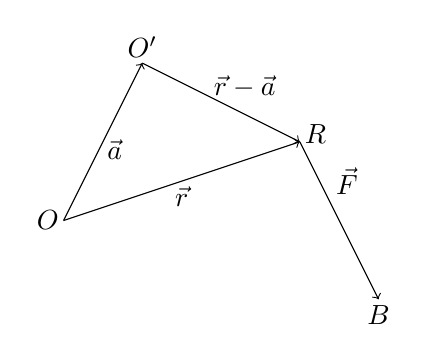
\begin{tikzpicture}
				\draw[->] (0,0)node[xshift=-0.2cm]{$O$} node[xshift=1.5cm,yshift=0.3cm] {$\vec{r}$} -- (3,1)node[xshift=0.2cm,yshift=0.1cm]{$R$};
				\draw[->] (3,1)node[xshift=0.6cm,yshift=-0.5cm] {$\vec{F}$} -- (4,-1)node[yshift=-0.2cm]{$B$};
				\draw[<-] (3,1) node[xshift=-0.7cm,yshift=0.7cm] {$\vec{r}-\vec{a}$} -- (1,2)node[yshift=0.2cm]{$O'$};
				\draw[<-] (1,2) -- (0,0)node[xshift=0.65cm,yshift=0.9cm] {$\vec{a}$};
			\end{tikzpicture}
		\end{center}
		Hence after shifting the origin the new torque ($\tau_f$) will be$$\tau_f=(\vec{r}-\vec{a})\times \vec{F}$$Hence the difference between final and initial torque is $$\tau_f-\tau_i=(\vec{r}-\vec{a})\times \vec{F}-\vec{r}\times \vec{F}=-\vec{a}\times \vec{F}= \vec{F}\times\vec{a}$$Therefore if the origin is shifted by $\vec{a}$ then the change in torques is $\vec{F}\times\vec{a}$.
		\item Let $$\vec{a}=a_1\hat{i}+a_2\hat{j}+a_3\hat{k}$$and$$\vec{b}=b_1\hat{i}+b_2\hat{j}+b_3\hat{k}$$Therefore
			\begin{align*}
				\vec{a}\times\vec{b}\ &=\begin{array}{|ccc|}
				\hat{i}&\hat{j}&\hat{k}\\
				a_1&a_2&a_3\\
				b_1&b_2&b_3
				\end{array}\\
				&=(a_2b_3-a_3b_2)\hat{i}+(a_3b_1-a_1b_3)\hat{j}+(a_1b_2-a_2b_1)\hat{k}
			\end{align*}Hence the cartesian components of $\vec{a}\times\vec{b}$ is $(a_2b_3-a_3b_2)\hat{i}+(a_3b_1-a_1b_3)\hat{j}+(a_1b_2-a_2b_1)\hat{k}$
		\item Let $$\vec{a}=a_1\hat{i}+a_2\hat{j}+a_3\hat{k}$$ $$\vec{b}=b_1\hat{i}+b_2\hat{j}+b_3\hat{k}$$ $$\vec{c}=c_1\hat{i}+c_2\hat{j}+c_3\hat{k}$$
		Therefore\begin{align*}
			\vec{a}\times\vec{b}\ &=\begin{array}{|ccc|}
				\hat{i}&\hat{j}&\hat{k}\\
				a_1&a_2&a_3\\
				b_1&b_2&b_3
			\end{array}\\
			&=(a_2b_3-a_3b_2)\hat{i}+(a_3b_1-a_1b_3)\hat{j}+(a_1b_2-a_2b_1)\hat{k}
		\end{align*}and\begin{align*}
		\vec{b}\times\vec{c}\ &=\begin{array}{|ccc|}
			\hat{i}&\hat{j}&\hat{k}\\
			b_1&b_2&b_3\\
			c_1&c_2&c_3
		\end{array}\\
		&=(b_2c_3-b_3c_2)\hat{i}+(b_3c_1-b_1c_3)\hat{j}+(b_1c_2-b_2c_1)\hat{k}
		\end{align*}Now\begin{align*}
			LHS=\vec{a}\cdot (\vec{b}\times\vec{c})\ &=(a_1\hat{i}+a_2\hat{j}+a_3\hat{k})\cdot\Big((b_2c_3-b_3c_2)\hat{i}+(b_3c_1-b_1c_3)\hat{j}+(b_1c_2-b_2c_1)\hat{k}\Big)\\
			&=a_1(b_2c_3-b_3c_2)+a_2(b_3c_1-b_1c_3)+a_3(b_1c_2-b_2c_1)\\
			&=c_1(a_2b_3-a_3b_2)+c_2(a_3b_1-a_1b_3)+c_3(a_1b_2-a_2b_1)
		\end{align*}
		and\begin{align*}
			RHS=\vec{c}\cdot (\vec{a}\times\vec{b})\ &=(c_1\hat{i}+c_2\hat{j}+c_3\hat{k})\cdot\Big((a_2b_3-a_3b_2)\hat{i}+(a_3b_1-a_1b_3)\hat{j}+(a_1b_2-a_2b_1)\hat{k}\Big)\\
			&=c_1(a_2b_3-a_3b_2)+c_2(a_3b_1-a_1b_3)+c_3(a_1b_2-a_2b_1)
		\end{align*}
		Therefore $LHS=RHS$. Hence$$\vec{a}\cdot(\vec{b}\times\vec{c})=\vec{c}\cdot(\vec{a}\times\vec{b})\ [\text{Proved}]$$
		\item Let$$\vec{a}=\hat{i}+2\hat{j}+3\hat{k}$$$$\vec{b}=2\hat{i}+3\hat{j}+4\hat{k}$$$$c=3\hat{i}+4\hat{j}+5\hat{k}$$
		Then\begin{align*}
			\vec{a}\times\vec{b}\ &=(\hat{i}+2\hat{j}+3\hat{k})\times(2\hat{i}+3\hat{j}+4\hat{k})\\
			&=(2\times4-3\times3)\hat{i}+(3\times 2-1\times 4)\hat{j}+(1\times3-2\times2)\hat{k}\\
			&=-\hat{i}+2\hat{j}-\hat{k}
		\end{align*}hence
	\begin{align*}
		(\vec{a}\times\vec{b})\times\vec{c}\ &=(-\hat{i}+2\hat{j}-\hat{k})\times(3\hat{i}+4\hat{j}+5\hat{k})\\
		&=(2\times5-(-1)\times4)\hat{i}+((-1)\times3-(-1)\times5)\hat{j}+((-1)\times4-2\times3)\hat{k}\\
		&=14\hat{i}+8\hat{j}-10\hat{k}
	\end{align*}
		and\begin{align*}
			\vec{b}\times\vec{c}\ &=(2\hat{i}+3\hat{j}+4\hat{k})\times(3\hat{i}+4\hat{j}+5\hat{k})\\
			&=(3\times5-4\times4)\hat{i}+(4\times3-2\times 5)\hat{j}+(2\times4-3\times3)\hat{k}\\
			&=-\hat{i}+2\hat{j}-\hat{k}
		\end{align*}hence
	\begin{align*}
		\vec{a}\times(\vec{b}\times\vec{c})\ &=(\hat{i}+2\hat{j}+3\hat{k})\times(-\hat{i}+2\hat{j}-\hat{k})\\
		&=(2\times(-1)-3\times2)\hat{i}+(3\times(-1)-1\times(-1))\hat{j}+(1\times2-2\times(-1))\hat{k}\\
		&=-8\hat{i}-2\hat{j}+4\hat{k}
	\end{align*}Therfore$$ (\vec{a}\times\vec{b})\times\vec{c}\neq \vec{a}\times(\vec{b}\times\vec{c})$$Hence the cross product is not associative. [Proved]

	\end{enumerate}

\end{document}